\section{How far can the data exclude a material class?}\label{sec:experiments}

All comparisons use $d/r$, where $d$ is an outward lower endpoint for the distance to a class and $r$ is its joint complex-field error radius. A ratio above one rules out the hypothesis. An upper endpoint for the \emph{method} below one shows that this test cannot decide. Only an admissible material with a full-wave residual at most $r$ establishes physical compatibility. Once a cap is excluded, the same conclusion holds for every smaller cap by nesting, even if a particular weight choice gives a smaller numerical bound there. We report the largest \emph{tested and excluded} cap. Interpolation in $u$ does not establish an optimal threshold.

For the computations, OpenAI Codex (GPT-6.2 Astra and Sol) assisted in deriving candidate bounds, implementing the full-wave calculations and selecting diagnostic comparisons. Google Gemini Neon independently inspected the physical operators and proposed tests of the negative-mode currents. The reported numerical inequalities use the deterministic arithmetic described in Appendix~\ref{app:tech}. Figures plot saved numerical arrays.

Table~\ref{tab:geometry} sets the physical scale. Each synthetic noise vector is a fixed circular complex Gaussian realization normalized to the stated fraction of the clean field norm. The principal error ball includes $10^{-6}\|Y\|_F$ to cover the error in generating the data. For the same material, array and loss comparisons are paired. Material maps enter the forward simulation and physical controls, but no map, current from a generating medium or support enters selection of weights, pixels or coherent directions.

\begin{table}[tbp]
\centering\small
\caption{Arrays and electrical sizes. The square of width $W$ has circumscribed radius $a=W/\sqrt2$. Incident fluence is fixed across the source sweep. The receiver count in the two chambers is per source or common-row group.}
\label{tab:geometry}
\begin{tabular}{@{}lrrrrr@{}}\toprule
Material family & Grid & GHz & $W/\lambda$ & $ka$ & Sources, receivers\\\midrule
Six lossless shapes & $96^2$ & 0.4 & 2.67 & 11.85 & 10--32, 20/32\\
Two compact lossy shapes & $12^2$ & 0.4 & 0.80 & 3.55 & 10, 20\\
Two wider lossy shapes & $12^2$ & 0.4 & 1.67 & 7.40 & 10, 20\\
Annular materials & $24^2$ & scaled & 0.96 & 4.27 & 12, 48\\
Austria target & $32^2$ & 0.4 & 2.67 & 11.85 & 20, 40\\
Fresnel & $60^2$ & 4--8 & 2.67--5.34 & 11.86--23.71 & 8/18, 241\\
Manitoba & $40^2$ & 3--6 & 1.40--2.80 & 6.22--12.45 & 12, 12\\\bottomrule
\end{tabular}
\end{table}

\subsection{When illumination diversity pays for a negative current}

Figure~\ref{fig:geometry} shows the six distributions sampled on the original grid. The domain is $2\,\mathrm m$ square. Receivers lie on a circle of radius $3.75\,\mathrm m$. The plane-wave amplitudes are multiplied by $\sqrt{10/s}$ and receiver samples by $\sqrt{20/p}$. Changing from ten to twenty-four shots at 2\% noise and $p=20$ raises the number of objects for which a peak above 0.75 is established from two to five. An increase from twenty-four to thirty-two leaves the count at five for either receiver density. The saturation is consistent with $2ka\simeq23.7$. The count also depends on the objects' source spectra. Graded pinwheel, for example, has insufficient retained energy on every one of these views.

\begin{figure}[tbp]\centering
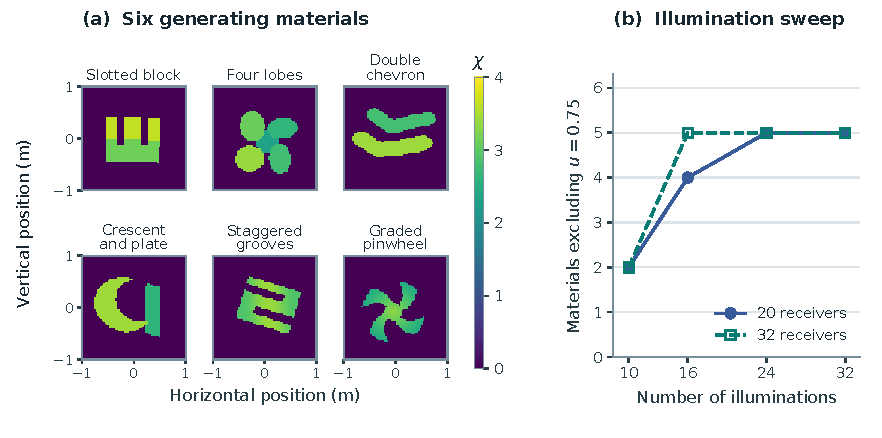
\includegraphics[width=.96\linewidth]{geometry.pdf}
\caption{The six independent dielectric distributions on a common contrast scale. At right, the number for which the measured data exclude a peak of 0.75, at equal total incident fluence and 2\% noise. Each point uses the same six objects.}
\label{fig:geometry}
\end{figure}

Half-ring reception leaves a substantial radiative component in the unmeasured current. On the native $96^2$ grid the leading numerical eigenvalue of $R_0$ is 4.805 for the half ring and 0.544 for the full ring, with $\|R\|_2\simeq5.095$ in the same units. For the denser receiver arrays of the compact annular and Austria tests, rigorous upper bounds on $\|R_0\|_2$ are respectively $7.56\,10^{-15}$ and $3.03\,10^{-10}$ in their own normalizations. At a cap of 0.5 and 2\% noise on the half ring, the tested real sector alone gives zero exclusions out of six. Adding optical balance gives six. At 10\% noise, adding quadrant balances to the global optical test increases the count from two to three. On the full ring the real sector already excludes 0.5 in all six cases at either noise level. These ablations fix the data within an aperture. In the comparison between apertures the illumination directions change as well.

At 2\% noise, ten incident fields and twenty full-ring receivers give a rigorous separation from tests with just one coherent combination. For Slotted block and Staggered grooves, the joint distances at cap 0.75 exceed 0.16069 and 0.11060, compared with radii 0.09097 and 0.08803. For each unit coherent input, a single current fits the receivers under both global balances. Under four regional balances and a uniform, physically necessary energy cap, a positive semidefinite lift also fits every coherent input exactly. Appendix~\ref{app:tech} gives the construction. With sixteen regions, particular coherent inputs do exclude the cap, at distances 0.18967 and 0.12452. The practical distinction depends on both the number of independently tested source directions and how much spatial variation the balances retain.

\subsection{Lossless media at increasing peak and electrical size}

On the 32-source, 32-receiver data at 2\%, one fixed, spatially constant profile excludes 0.78125 on five objects, 0.8125 on three, and 0.84375 on Crescent and plate alone, where $d/r>1.31$. These are improvements in resolution of the cap sweep using the rank bound. Several intervening or larger caps could not be settled by the selected Fourier floor. We show them as unresolved. At cap one the strongest previously evaluated scalar profile on these six data has $\nu=13$. In units of its scale $\mu=1.3535749382\,10^{-5}$, the negative and positive gaps exceed 0.03017 and 0.0019531. The source basis is 32-dimensional. Directly retaining the source eigenvalues gives at most $0.30106r$ on the six cases. Maximizing each ordered lower eigenvalue separately over the available profiles brings this to $0.30604r$ as a lower endpoint.

\begin{figure}[tbp]\centering
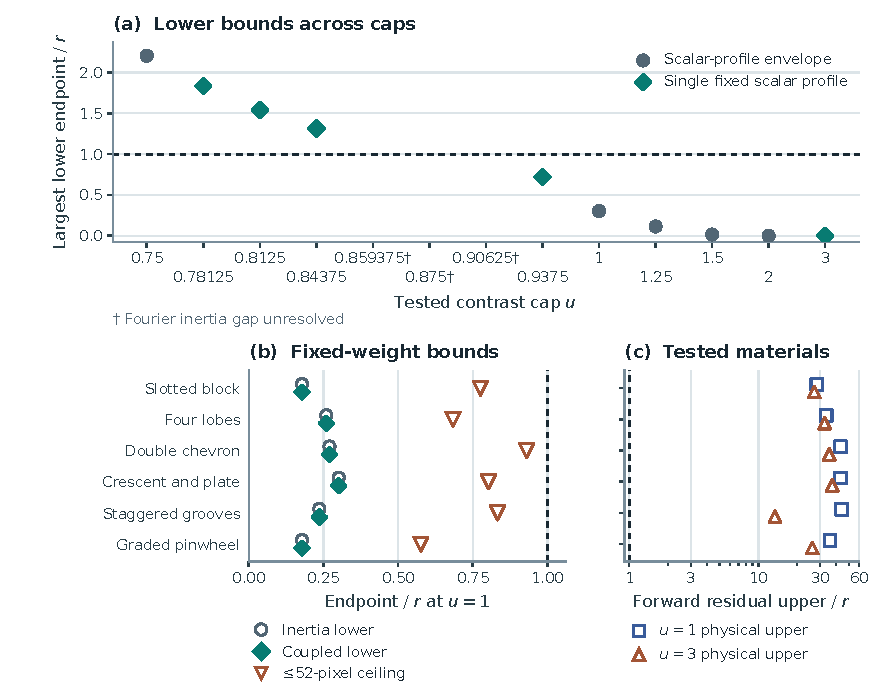
\includegraphics[width=\linewidth]{full-domain.pdf}
\caption{Lossless contrast tests on the full search square. Measured lower distances, upper limits on a family of local tests and residuals achieved by actual box-constrained materials answer three distinct questions. Missing spectral enclosures are indicated separately. The threshold line is the radius of the same data ball for all methods on one object.}
\label{fig:whole}
\end{figure}

We first attempted to recover source eigenvalues by local compensation on the same operator. The full positive spectrum was eliminated using the row Gram in Appendix~\ref{app:tech}. Rows were proposed by rank-revealing QR on negative-mode endpoint responses. For the 52-row calculation, the 104-by-104 endpoint Gram upper enclosure required an upward shift below $4.75\,10^{-9}$ in its normalized units. A center-aware semidefinite fit, including interval constraints on every selected material, gave $d/r>0.30104$ for Crescent and plate. The rank bound already gave $d/r>0.30105$. Failure of that particular selection did not settle whether other pixels could do better.

Applying Proposition~\ref{th:obstruction} to the \emph{entire} pixel pool gives a different conclusion. At an admissible material, the trace on the full negative space is below 0.98227 for any 29 separately weighted constitutive rows and below 1.98201 for any 59. Thus the former can compensate no negative direction and the latter at most one. This conclusion follows by sorting bounds for all 9,216 cells. Including the center with either sign of $M_Y$, Table~\ref{tab:scope} gives upper endpoints at 52 cells. At 59 cells the largest upper endpoint among the six is still below $0.97803r$. These counts refer to this grid, these state weights and nonnegative weights on individual constitutive rows. The computations also allowed a coupled positive semidefinite metric on each of three specific nested row sets of sizes 8, 26 and 52. The smallest eigenvalues of their signed row Grams exceeded 0.9790, 0.9471 and 0.8335 for suitable uniform test materials. None can uniformly compensate one negative direction, including after retaining additional positive modes explicitly in the local row calculation.

\begin{table}[tbp]\centering\small
\caption{Same native data and cap $u=1$. The first two columns are attained lower endpoints divided by $r$ at the same fixed current weights. The third is an upper endpoint on \emph{any} diagonal local compensation bound using at most 52 cells including signed center corrections. The fourth is the residual upper endpoint of an actual candidate material. The last two columns bound different mathematical quantities.}
\label{tab:scope}
\begin{tabular}{@{}lrrrr@{}}\toprule
Object & Rank & All-cell defect & 52-cell limit & Trial residual\\\midrule
Slotted block & .17833 & .17839 & .77551 & 28.330\\
Four lobes & .25949 & .25957 & .68392 & 33.363\\
Double chevron & .27019 & .27035 & .93030 & 43.231\\
Crescent and plate & .30105 & .30115 & .80274 & 43.154\\
Staggered grooves & .23632 & .23640 & .83274 & 44.094\\
Graded pinwheel & .17837 & .17850 & .57643 & 35.752\\\bottomrule
\end{tabular}
\end{table}

On larger selected sets of 208 and 416 cells the trace comparison gives $c\le3$ and $c\le4$, respectively. Even an ideal zero center charge would require $c\ge7,5,5,5,5,7$ in object order to reach the data radius. These last impossibility conclusions use $M_Y\succeq0$. Allowing all 9,216 cells still gives $c\le8$ for diagonal nonnegative frames at these weights. A second test retained two, four or eight weak positive current modes explicitly before bounding the remainder by a uniform Young inequality. Even after optimizing its scalar split, the number of compensated directions cannot exceed two, two or three, respectively, on this fixed split. A zero or nonnegative center charge would require at least five. Results for signed charges beyond the proved cardinality range and for freely varying frames remain open. At cap 1.25 another fixed profile has fifteen negative directions. Any 60 local rows have $c=0$, and up to 30 cannot yield an exclusion on any object even with a signed center.

We then used the full-box calculation \eqref{eq:full_def} with all cells. Choosing $\omega/\mu=10^{-3}$ and $\eta/\mu=2^{-20}$ preserves the index bound of thirteen and increases all six source lower endpoints slightly (Table~\ref{tab:scope}). The large local constitutive defects in the strongest illumination directions contribute little here because the first thirteen source eigenvalues are lost to interlacing. More aggressive weights spend additional negative directions and lose further source eigenvalues. This trade is present on the original grid and survives interval evaluation of the full stationary currents. In parallel, nonlinear box-constrained fits were initialized by coarse material updates, bounded Gauss--Newton, projected gradient and contrast-source inversion. Across eighteen object--cap combinations up to $u=3$ the best candidate in each tried combination was replayed by an independent full-grid state solve. At $u=3$ their smallest residual upper endpoint is $13.408r$. The lower sides of the individual fit residual intervals also exceed $r$. No search established physical feasibility under these caps. No lower-bound calculation at $u=1$ excluded them. A separately generated disk of peak 0.625 on the $96^2$ grid passes the $u=0.75$ physical control at $0.99995r$.

Changing the state weights offers a separate test. Divide the square into sixteen equal tiles and multiply the sector weight on the twelve outer tiles by 1.5 or 2.5, leaving the four central tiles and optical weight unchanged. All material pixels remain unknown. The exact full-state negative counts fall from thirteen to eleven and eight. The largest $d/r$ rises from 0.30105 to 0.31134 and 0.32376, respectively. For the second weight the projection onto the original thirteen modes counts only five negatives. Combining that count with the full source matrix gives spurious numerical threshold crossings on five objects. Even where the projected count agrees at the first weight, using its projected stationary field gives apparent ratios between 2.27 and 6.24 on all six. The full calculation puts every one below 0.312. Both errors result from truncating the current state before changing the quadratic. Reflection symmetry allows all four parity sectors of the actual operator to be checked without a material symmetry assumption (Appendix~\ref{app:tech}).

The same six unresolved observations do constrain which currents a successful reconstruction would have to contain. Setting the actual current component on the negative eigenspace to zero makes a cap-one fit impossible on \emph{all six} objects. The lower endpoints in \eqref{eq:required} for its Frobenius norm, in object order, are 15.75, 9.05, 14.42, 22.00, 19.76 and 7.65 in the unweighted discrete current coordinates. With zero such current the measured source forms alone would require residuals above $1.19r$ on every object. This rules out an exact truncation of that specific state subspace within the tested cap, even though the complete cap remains open. A legal cap-one candidate for Slotted block has negative current norm above 41.85 and misses the measured ball. Therefore any data-independent scalar upper norm valid over the whole box must allow at least that much current. The particular lower norms obtained here cannot be turned into full material exclusions by imposing a smaller scalar ceiling. The independent low-peak disk has negative current norm 18.39956 in its own error ball. A physical scatterer can drive these modes at modest contrast (Figure~\ref{fig:modes}).

\begin{figure}[tbp]\centering
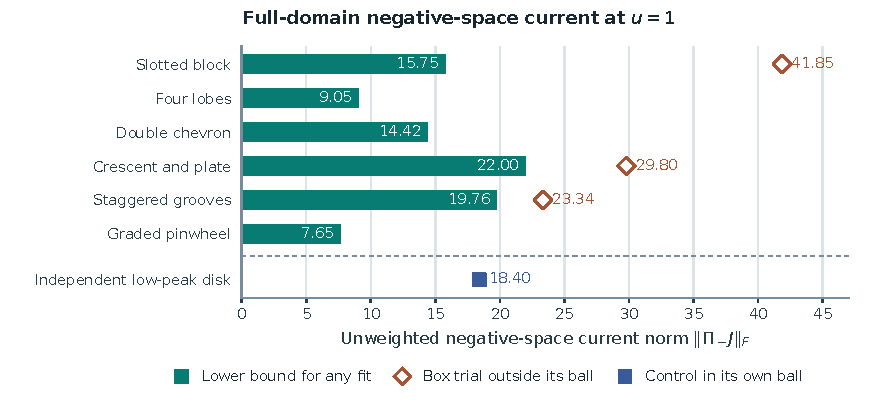
\includegraphics[width=\linewidth]{current-modes.pdf}
\caption{How much of the physical current must occupy the 13 negative modes at a contrast cap of one? Bars give lower bounds for any fit to the six observations. Open symbols mark full-wave currents of three box-admissible candidates outside their measured balls. The square marks a low-peak control which fits its own data. All amplitudes use the same total incident fluence and unweighted discrete current norm.}
\label{fig:modes}
\end{figure}

Compact media show why the domain matters. On a separate, electrically smaller $24^2$ annular problem with twelve illuminations and four negative modes, one unchanged profile excludes a peak of five on five of seven independent materials at 1\% noise, with ratios 5.12--10.77. One of the other two really does fit below cap five, with a peak of 4.28. On twenty-two additional $96^2$ lossless objects with 10\% noise the joint calculation excludes 0.5 on all twenty-two, whereas none clears 0.75. These transfers cover different independently generated materials. A native result on a compact search region cannot be used as a uniform bound for a larger one.

\subsection{What a specified loss or a calibrated instrument adds}

The dissipative comparison uses new full-wave observations for every $t\in\{0.01,0.05,0.2\}$. Two fresh distributions were generated in each of two domain widths. All pixels remained free in the inverse problem. Figure~\ref{fig:diss} compares bounds at fixed material law, using identical data and noise radius. On the $0.6\,\mathrm m$ square at $t=0.2,u=1$, the two receiver-ellipsoid lower endpoints are $1.17917r$ and $1.23174r$. For the first material $r=0.05609216459$. A single interval calculation over \emph{all} common nonnegative penalties and optimal coherent source projectors gives $d<0.99873r$. The same physical information thus suffices or fails to exclude a material class depending on how its source dependence is retained. Even a fixed right-singular basis of $Z_Y$, with separate scalar penalties, gives $d>1.14159r$ and $d>1.10601r$ for the two objects. Applying separate penalties in the original illumination basis gives only $0.57351r$ for the first object.

\begin{figure}[tbp]\centering
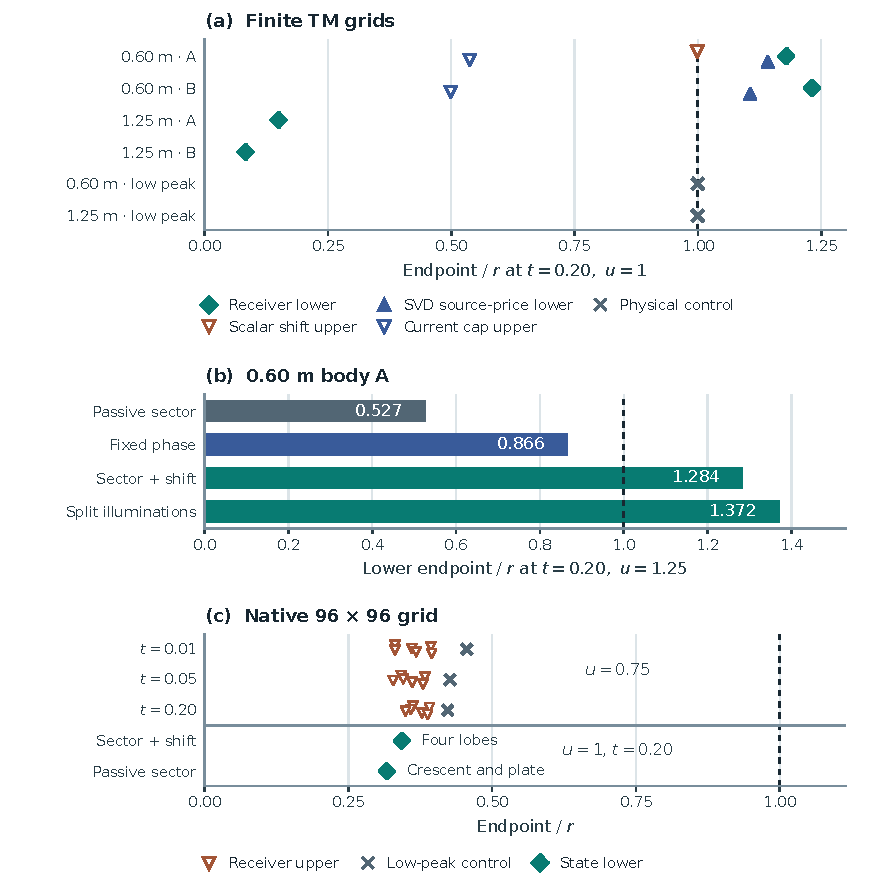
\includegraphics[width=\linewidth]{dissipation.pdf}
\caption{Bounds on the real contrast for specified loss tangents. Comparisons at the same loss tangent use the same complex data. Feasible points of a receiver ellipsoid upper-bound its distance, while only the verified low-peak material establishes a physical fit.}
\label{fig:diss}
\end{figure}

At the smaller loss tangent $t=0.05$ and cap $u=0.75$ the first object gives a wider separation. Subdivision of the complete common-penalty half-line gives a distance below $0.80975r$, while independent penalties in a fixed coherent basis give a lower bound above $1.01323r$. Direct projection raises this to $1.02003r$. On the second object the receiver distance is below $0.94901r$. At $t=0.2,u=1.25$ a whole-current dissipation shift \emph{combined with the sector} gives $d>1.28439r$ on the first object. The full receiver ellipsoid here has a distance below $0.66362r$. Using the same sector weights on a joint source block and independent receiver penalties on the orthogonal block raises the lower bound to $1.37213r$. After separately improving the sector weights, the matched whole-sector bound and the split give $1.51977r$ and $1.59135r$. These compare attained sector choices. At the higher cap 1.5 neither object is ruled out. For the first, the split reaches $0.61127r$ and the whole receiver ellipsoid alone gives more than $0.65218r$. For the second, the split reaches $0.72916r$, exceeding both the whole-sector result $0.59887r$ and the receiver distance upper endpoint $0.61437r$. The partitions were proposed using the measured source spectra and verified on the original matrices. The search scored all $2^{10}-2$ nonempty proper subsets in each of two data-derived coherent bases. An exhaustive subset search would grow exponentially with source count. At $u=1,t=0.2$ on the $1.25\,\mathrm m$ square, the two relaxed receiver distances are below $0.151r$ and $0.084r$. Finally, on the six $96^2$ shapes, even the tightest tested cap of 0.75 admits a receiver-ellipsoid point within $0.395r$ for each of the three loss tangents. Nesting proves that receiver projection alone cannot exclude any larger cap on those observed data. This statement concerns the exact outer sets. It does not produce a low-peak material.

For the finite examples one right-singular basis and its scalar solves cost 0.88 ms of CPU for the first object at $t=0.2,u=1$, after the common port Grams and bases had been formed. Direct iterative projection reached its 2,500-iteration limit after 0.319 s of CPU and supplied a valid dual direction. These figures exclude the shared setup and the separate interval evaluation and describe the computation of a proposal. On the larger array the corresponding median CPU times were 2.2 ms and 1.19 s. The six paired compact source-partition tests and their interval evaluations took 10.30 s wall time and 9.86 s CPU. An independent check of the positive spectral gaps added 0.54 s wall time and 0.52 s CPU. Detailed costs, including unsuccessful fits, are given in Appendix~\ref{app:tech}.

Two laboratory datasets set a separate limit on interpreting any positive lower bound. With measured total minus incident fields for the three Fresnel cylinders at 4, 6 and 8 GHz, none of the nine views clears the held-out empty-scene scale at a cap of 0.5 \cite{fresnel}. At cap 0.25 the twin target at 4 GHz leaves $6.98\%$ of the receiver norm for additional discrepancy after budgeting additive error and gain. In Manitoba four physical objects at seven frequencies are compared under four receiving calibrations \cite{manitoba}. Subtracting the largest displacement among these calibrations leaves a positive allowance in 20, 5, 3 and 1 of the 28 views at passive disk caps 0.25, 0.5, 0.75 and 1. The large nylon cylinder at 3 GHz leaves $4.018\%$ at cap one. These are explicitly conditional margins. Neither laboratory supplies a uniform bound on loaded-scene error for every hypothetical medium.

The same distinction matters when changing the object of the test. A sixteen-region localization test with unconstrained surroundings gave zero positive local bounds in 112 regional cases. A principal block in the exterior alone supplied enough negative directions to exhaust all available illuminations for the specified weight range. In a joint 400/500 MHz half-aperture comparison, three of six nominal low-cap decisions from separate frequencies became zero of six after adding the measured coarse-grid discrepancies. Conversely, enlarging a contrast range after ruling out a low peak on a compact patch reduced held-out complex-field error from 27.50\% to 1.32--2.52\%, while final relative material error rose from 0.462 to 0.721--0.943. An ordinary discrepancy stopping rule recovered much the same final fit. A full-class exclusion is a useful statement about the data even in a case where it gives no advantage in image accuracy.
\FloatBarrier

